\documentclass[journal]{IEEEtran}
\usepackage{cite}
\usepackage{placeins}
\ifCLASSINFOpdf
 \usepackage[pdftex]{graphicx}
  % declare the path(s) where your graphic files are
 \graphicspath{{Pics/}}
  % and their extensions so you won't have to specify these with
  % every instance of \includegraphics
  \DeclareGraphicsExtensions{.pdf,.jpeg,.png}
\else
\fi
\hyphenation{op-tical net-works semi-conduc-tor}
\begin{document}
\title{Ultra Low Energy Microcontroller Architectures}
\author{Aditya Tandon,~\IEEEmembership{at3g10@sotn.ac.uk,~University of Southampton} 
\thanks{}}
% The paper headers
\markboth{Individual Research Review} %
{Shell \MakeLowercase{\textit{et al.}}: Bare Demo of IEEEtran.cls for Journals}
\maketitle

\begin{abstract}
%\boldmath
The abstract goes here.
\end{abstract}
\IEEEpeerreviewmaketitle

\section{Introduction}
\IEEEPARstart{T}{his} report looks into low power and energy techniques for processor architectures 
 
\hfill \today

\section{Asynchronous design}
In a field of sensor networks asynchronous processors and microcontrollers have been gaining popularity as they lead to energy efficient designs. The basic principle is that these designs function without a global clock and hence reduce the number of unwanted switching activities in the circuit \cite{SNAP/LE}, \cite{LowPower2005}. To compensate for no clock, the designs usually employ extra hardware for a handshaking protocol \cite{SNAP/LE}. To further conserve energy these designs are event driven \cite{SNAP/LE}, \cite{LowPower2005}, \cite{AVR}. In such a system, the controller is mostly in a state of sleep until it is asked to perform a computation by an event. After performing the task the controller goes back to a sleep state thereby minimizing its active energy \cite{SNAP/LE}, \cite{LowPower2005}. Research has shown that there is no necessary software overhead for these systems due to their event driven nature \cite{SNAP/LE}, \cite{LowPower2005}. This is because these microcontrollers are used for a set of pre-defined tasks and can be simplified. For example, interrupts can be processed as events and there is no overhead to handle concurrent tasks \cite{SNAP/LE}, \cite{LowPower2005}. Designs can be further simplified by employing an in-order design which reduces the amount of hardware and therefore the amount of energy \cite{LowPower2005}, \cite{SmartDust}. \\

It can be observed that event driven architectures should have a minimal transition time from a sleep state to an active state. The SNAP/LE architecture addresses this concern by employing an event queue \cite{SNAP/LE}. This resembles a FIFO handler and tasks are executed if there is an event token present in the queue. If there is a token, the appropriate event handler associated with the token is looked up and the task is executed. After executing the task the processor goes into a 'sleep' state if there is no token present \cite{SNAP/LE}. The time taken by the processor to transition between an active and sleep state is the time taken for a token to go through the event queue \cite{SNAP/LE}. The length of the queue can be optimized so that this process is in the order of tens of nanoseconds and therefore this procedure saves energy and is also efficient \cite{SNAP/LE}. \\

Typically these designs can be modularised and stress can be taken off the microcontroller by employing hardware accelerators \cite{SNAP/LE}, \cite{LowPower2005}. Hempstead et al. \cite{LowPower2005} used the microcontroller only for computational intensive tasks and a separate event processor was employed which was effectively a hard-coded state machine to handle events which required light computation. This reduced the active and leakage power of the main controller. Another type accelerator used was the Message Coprocessor which was responsible for forming and forwarding incoming messages from the radio unit. Timing operations commonly found in wireless applications can be handled by a Timer Coprocessor and therefore can lead to a simplistic, energy efficient implementation for the microcontroller at the expensive of some additional hardware \cite{LowPower2005}. An architectural implementation of such a system can be seen from Figure \ref{Figure:Async}. \\
	
	\begin{figure}[h]
	   \centering
	   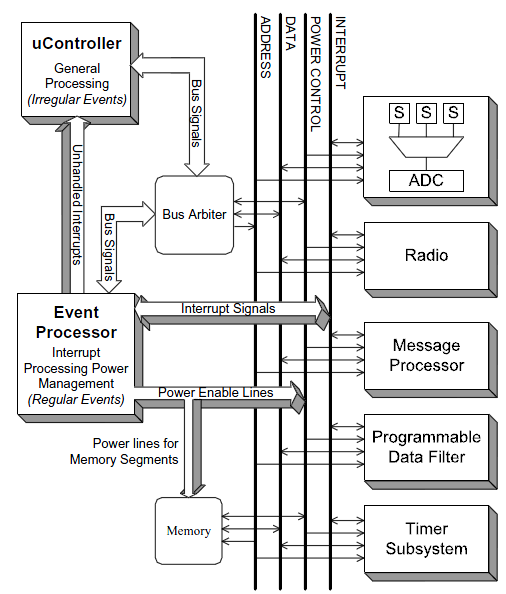
\includegraphics[width = 8cm]{Async}
	   \caption{Event driven design (reproduced from \cite{LowPower2005}).}
	   \label{Figure:Async}
	\end{figure}	
	\FloatBarrier
	
The steps taken in desynchronization involve replacing the clock tree with local, asynchronous controllers and converting the flip-flops into latches \cite{AVR}. This was demonstrated by Neechi et al. \cite{AVR} where a synchronous AVR microcontroller was used as a template to create an asynchronous version. It was found that the asynchronous controller was about 5 times more energy efficient than the synchronous one \cite{AVR}. The amount of energy that these prototype processors have taken to execute a particular instruction has been in the range of 10pJ – 14pJ assuming an operating voltage of 1.2V and about 2.7pJ/instruction at 0.54V \cite{SNAP/LE}, \cite{AVR}, \cite{SmartDust}.
	 
\section{Low power memory}
Over the years researchers have come up with different techniques to mitigate energy loss due to memory. A proposal for an adaptive cache for mobile processors could help reduce power \cite{Mem-Cache}. The L2 caches on mobile phones have been found to have access patterns that are not correlated or balanced and therefore there is scope to dynamically adjusting the cache to match the application using it \cite{Mem-Cache}. The compiler does an offline analysis of the application before run-time to determine parameters such as global average miss rates and access rates. Cache access is also monitored during run-time and the run-time information in conjunction with the offline material is used to enlarge or decrease the size of the cache dynamically depending on the need \cite{Mem-Cache}. This proves useful as memory is used much more efficiently. Also, the leakage power is reduced as there are fewer idle cells. This technique was found to give a 13\% - 29\% reduction in power consumption (using benchmark programs) but there was a small trade-off for speed and area to incorporate this \cite{Mem-Cache}.\\

	\begin{figure}[h]
	   \centering
	   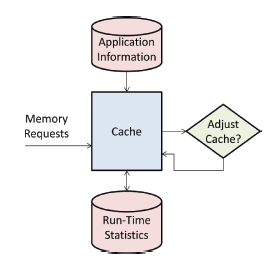
\includegraphics[width = 5cm]{AdaptiveCache}
	   \caption{Adaptive cache design (reproduced from \cite{Mem-Cache}).}
	   \label{Figure:Mem-Cache}
	\end{figure}	
	\FloatBarrier

Another technique to reduce power is memory compression \cite{MemComp}. Here, a part of the data in volatile memory is compressed in order to reduce the number of logic elements that have to be self-refreshed when a device is turned into a low power state. Rest of the memory can be powered off and therefore the battery life is extended \cite{MemComp}. When there is a request to put a device into a low power state, the memory compression logic takes blocks from a designated memory, compresses it using a compression algorithm and then stores these blocks back to memory. A decompression procedure is followed when the device is in the active state \cite{MemComp}. The compression logic can be implemented in hardware or software and induces some overhead on the battery while performing compression but the power saved by compressing data outweighs this overhead \cite{MemComp}.\\

Non-volatile memories are another area of interest for power reduction and even in performance enhancement \cite{NonVolatile}. Resistive Random Access Memory (RRAM) is a piece of memory that could be used as a substitute for SRAMs on mobile devices \cite{NonVolatile}. It was found that an RRAM with a crosspoint structure that uses a diode as a select cell reduces leakage current. This is because the resistance goes up as voltage decreases and the leakage current paths are cut-off \cite{NonVolatile}. This structure is also area efficient as multi-layered structures can be made \cite{NonVolatile}. Investigation is still going into this area as peripheral circuit design is harder if RRAMs are used but it could be used as a technique to reduce energy and power \cite{NonVolatile}.\\

Many other techniques can be used to reduce power. An Intel processor for mobile devices reduces the leakage power in the L2 cache \cite{Intel}. The data arrays in the cache continue to be in the ‘sleep’ mode until a ‘Hit’ signal is generated. Even when there is a hit, only the relevant data array is charged so that it can be activated while the other arrays continue to be in the low power mode \cite{Intel}. This is a memory partitioning technique and is widely used to mitigate leakage power \cite{LowPower2005}, \cite{Intel}.
\section{Subthreshold design}
Devices operating in the subthreshold region show a reduction in energy because the switching activity decreases with supply voltage \cite{FFT}. However, the propogation delay increases in this region and this gives rise to leakage currents which cause energy dissipation \cite{FFT}. There exists an optimal operating point in the subthreshold region at which devices can operate. This point can be found through a minimum energy analysis technique in which the energy is plotted against the supply voltage as the voltage is scaled down \cite{FFT}. Wang and Chandrakasan \cite{FFT} implemented this idea in a FFT processor to demonstrate how devices can operate in subthreshold regions. Logic elements have to be specifically modified to be catered for subthreshold operation to avoid leakage current. Parallel leakage is a major contributor to leakage current and it occurs when the idle current is comparable to the drive current in circuits \cite{FFT}. This effect can be mitigated by having reducing or balancing the number of parallel devices in the pull up and pull down path to avoid leakage \cite{FFT}. Devices should avoid being stacked as this reduces the effective drive current of each transistor in a stack \cite{FFT}. \\

RAM blocks usually contain six transistor (6T) scheme to enable reading and writing of data. Wang and Chandrakasan have demonstrated that subthreshold conditions make read and write operations harder as they place a sizing constraints on the transistors used \cite{FFT}. There are also other considerations such as bitline leakage that comes into effect when operating in this region \cite{FFT}. Therefore, an alternative structure to the RAM is needed to address this problem. In the FFT processor, the RAM uses tristate inverters to create a latch and this is used for write operations. The read operation uses parallel tristate gates and a hierarchical read bitline to mitigate parallel leakage \cite{FFT}. \\

Therefore, it can be observed that operating in the subthreshold region can help in energy savings but only if the logic is suitably catered for it. Designers might have to construct subthreshold libraries if they want their devices operating in this region. The gains in the long run are satisfactory as it results in an energy efficient device.  The subthreshold FFT chip that was made was found to be ``350 times more energy efficient than the low-power microprocessor implementation'' which was a microprocessor that did not include subthreshold logic \cite{FFT}.


\section{Power management schemes}
\subsection{Power management}
Chips on mobile phones are now moving towards a multi-core implementation to support the vast functionality that is in demand. The cores are usually heterogenous so that each of them can run at an independent frequency and hence utilized in the best possible way and also reduce dynamic power \cite{HierarchicalPower}. A single chip implementation makes it hard for power management schemes to achieve power reduction due to leakage currents. A multi-chip scheme paves way to implementing a partial power off scheme where unused chips can be powered off if they are not in use \cite{HierarchicalPower}. This gives rise to the concept of a power domain where different parts of a chip and also different chips can be isolated from each other in terms of power management \cite{HierarchicalPower}. Many domains can thus be created and power can be saved. Implementing power domains does pose some problems. For example, the shutdown elements between power domains need to be robust and reliable \cite{HierarchicalPower}. µI/O’s are used to route signals from domains that might be powered off. These are special circuits used to isolate such signals \cite{HierarchicalPower}. To minimize such additional signals, a hierarchical power domain scheme can be adopted which sets a level of precedence for certain domains \cite{HierarchicalPower}. So no µI/O’s are needed from a higher hierarchy to a lower one as the lower hierarchy cannot be on while the upper one is switched off. Figure \ref{Figure:Hier} illustrates a hierarchical structure that can be implemented on mobile phones.

	\begin{figure}[h]
	   \centering
	   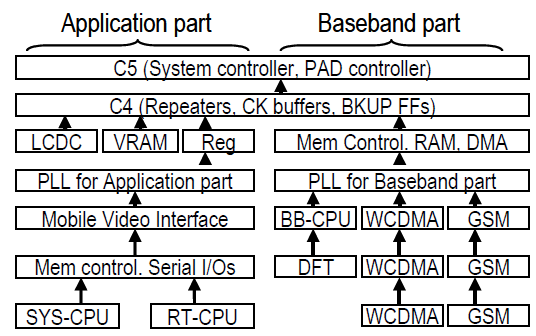
\includegraphics[width = 7cm]{Hier}
	   \caption{Hierarchical power domains (reproduced from \cite{HierarchicalPower}).}
	   \label{Figure:Hier}
	\end{figure}	
	\FloatBarrier

Another problem is the rush current generated while switching on power domains \cite{HierarchicalPower}. Hattori et al. \cite{HierarchicalPower} described an efficient power switch design to minimize this rush current so that it can be made negligible. They observed very low leakage currents using this design and so the use of hierarchical power domains could be an effective way to save energy \cite{HierarchicalPower}. \\

Power gating is another strategy that has been around for quite a while. Here, the processor is switched off due to switches inserted into the power rail \cite{LDO}. This causes a reduction in power but there are other components, such as state retention registers, power management unit and Low Drop Regulator (LDO) still remain active and contribute to leakage current \cite{LDO}. To mitigate this, Lueders et al. \cite{LDO} proposed a scheme based around the LDO. The idea was that a digitally adaptive LDO would drive the micro-controller unit and based on the requirements, it would adapt its drive current and hence reduce power management overhead in low frequency operations \cite{LDO}. Also, as the LDO is integrated onto the chip, it would be designed with a low output capacitance and therefore take up very little power during sleep and also have a quick transition wake up time \cite{LDO}. During sleep mode, the LDO can be disabled and it was shown that a power saving of a factor of 4.3 was achieved as compared to power gating \cite{LDO}. This was easier to implement than power gating as system partitioning was simple and no power switches had to be used \cite{LDO}. \\

Other power management schemes, include the implementation of different power states in a system \cite{Intel}. For example, an Intel processor for mobile phones has 6 power states (C0 – C6) \cite{Intel}. The C0 state is the high frequency state and in C6 state the core power is shutdown \cite{Intel}. The intermediate states involve the power gating of different components such as the core clock, phase locked loops and flushing of L1 caches to reduce dynamic power \cite{Intel}.   


\subsection{Dynamic voltage and frequency scaling}

Dynamic voltage and frequency scaling (DVFS) is used ubiquitously to improve energy performance in processors \cite{LinuxGov}, \cite{TempDVFS}, \cite{48Core}. Power is proportional to frequency and the square of supply voltage so scaling down these parameters saves energy \cite{TempDVFS}. Although delay increases with a reduced voltage so applications that are not time critical can be performed at a lower voltage to avoid performance hits \cite{LinuxGov}. Multicores on mobile phones can be made much more energy efficient if they ran at an optimum operating point. This operating point is a combination of choosing the correct operating frequency and the number of cores used for an application \cite{LinuxGov}. Quite often, cores are under-utilized in order to save energy but this actually dissipates more energy as fewer cores are running intensive programs at a higher frequency. Instead of this, more cores can be made available and can operate at a lower frequency \cite{LinuxGov}. This increases the number of computation resources and also reduces the energy as the operating frequency is low. Also, the work gets executed faster and power dissipation outside the cores can be minimized as these components can be turned off once the computation is finished \cite{LinuxGov}. Carol and Heiser \cite{LinuxGov} have come up with a linux governor that actually implements this concept. Frequency is increased if a core is being over-utilized and vice versa. It also disables and enables cores based on their need and this could be a useful tool to incorporate onto devices as an energy saving of upto 25\% was observed in this case \cite{LinuxGov}.\\

Dynamic Thermal Management (DTM) is another important aspect to consider when discussing DVFS \cite{TempDVFS}. If the temperature of a chip exceeds a certain thermal threshold the frequency has to be scaled down again to prevent the chip from over-heating. Once the temperature goes down the frequency is increased again and this would result in the thermal threshold being exceeded \cite{TempDVFS}. It can be observed that in some scenarios the operating frequency can oscillate between two frequencies due to DTM and this causes a degradation in power as the chip operates at an unstable frequency \cite{TempDVFS}. To mitigate this, Kim et al. \cite{TempDVFS} proposed a DVFS scheme based on an average frequency operating point so that the frequency is stable. Frequencies are sampled on a periodic basis when they exceed the thermal threshold and an average is formed once enough samples are collected \cite{TempDVFS}. This operating point can be re-sampled for different criteria if, for example, the frequency needs to be lowered or raised. This can lead to a reduction in energy and an energy saving of 12.7\% was observed in this scheme \cite{TempDVFS}.


\section{Other techniques}
\begin{itemize}
	\item Adaptive Body Bias: FBB to improve performance and RBB to reduce power. Only applied to parts of the chip \cite{ABB}
	\item Heterogeneous multicores and understanding the connections between hardware and software \cite{HD/SF} \cite{MultiCores}
	\item Low power FPGA on mobile phones: power gating per tile, low leakage SRAM and other techniques to reduce power \cite{FPGA}
\end{itemize}

\section{Conclusion}
The conclusion goes here.

\appendices

\section*{Acknowledgment}
The authors would like to thank...


% Can use something like this to put references on a page
% by themselves when using endfloat and the captionsoff option.
\ifCLASSOPTIONcaptionsoff
  \newpage
\fi


\bibliographystyle{IEEEtran}
% argument is your BibTeX string definitions and bibliography database(s)
\bibliography{IEEEabrv,References}

\end{document}